\documentclass{beamer}
\mode<presentation> {%
	\usetheme[]{Boadilla}
	\usecolortheme{orchid}
	\setbeamercovered{transparent}
	\setbeamersize{text margin left=0.7cm}
  \setbeamersize{text margin right=0.7cm}
  \setbeamertemplate{enumerate item}[square]
  \setbeamertemplate{enumerate subitem}[circle]
  \setbeamertemplate{enumerate subsubitem}[>]
  \setbeamertemplate{itemize item}[square]
  \setbeamertemplate{itemize subitem}[circle]
  \setbeamertemplate{itemize subsubitem}[>]
}

\usepackage[utf8]{inputenc}
\usepackage[spanish]{babel}
\usepackage{graphicx}
\usepackage{amsmath}
\usepackage{listings}
\usepackage{xcolor}

% \usepackage{booktabs}
\definecolor{codegreen}{rgb}{0,0.6,0}
\definecolor{codegray}{rgb}{0.5,0.5,0.5}
\definecolor{codepurple}{rgb}{0.58,0,0.82}
\definecolor{backcolour}{rgb}{0.95,0.95,0.92}
\definecolor{olivegreen}{rgb}{0.0,0.5,0.0}
% \definecolor{general}{rgb}{0.9 0.9 1}%
% \newrgbcolor{colorsistema}{0 1 1}
% \newrgbcolor{colorviolet}{0.9 0.8 1}

\lstdefinestyle{mystyle}{
    backgroundcolor=\color{backcolour},
    commentstyle=\color{codegreen},
    keywordstyle=\color{magenta},
    numberstyle=\tiny\color{codegray},
    stringstyle=\color{codepurple},
    basicstyle=\ttfamily\footnotesize,
    breakatwhitespace=false,
    breaklines=true,
    captionpos=b,
    keepspaces=true,
    numbers=left,
    numbersep=5pt,
    showspaces=false,
    showstringspaces=false,
    showtabs=false,
    tabsize=2
}

\lstset{style=mystyle}


\title[Procesamiento de Señales]{Transformada de Fourier Discreta (DFT)}
\author[J. Chacón]{%[Author, Another] % (optional, use only with lots of authors)
\textit{Ingeniería Electrónica de Comunicaciones }\\
\vspace{0.6cm}
\small Jesús Chacón Sombría}

\institute[DACYA] % (optional, but mostly needed)
{
  %\inst{1}%

\footnotesize  Departamento de Arquitectura de Computadores y Automática.\\
  Universidad Complutense de Madrid
  }

\date[Transformada Fourier Discreta] % (optional)
{\footnotesize Curso 2025-2026}%{\today / Master}
\subject{Talks}

\pgfdeclareimage[height=0.75cm]{logo}{ucm.png}

\usepackage[absolute,overlay]{textpos}
\setlength{\TPHorizModule}{1mm}
\setlength{\TPVertModule}{1mm}
\newcommand{\MyLogo}{%
\begin{textblock}{14}(116.0,0.6)
  \pgfuseimage{logo}
\end{textblock}
}

\makeatletter
\numberwithin{section}{part}
\AtBeginPart{
\beamer@tocsectionnumber=0\relax
\frame{\partpage}
}
\makeatother

\begin{document}

\begin{frame}
  \titlepage
\end{frame}

\newcommand*\oldmacro{}%
\let\oldmacro\insertshorttitle%
\renewcommand*\insertshorttitle{%
 \MyLogo
  \oldmacro\hfill%
}

\AtBeginSection[]{}

\AtBeginSubsection[]{}      


\section{Introducción}
\begin{frame}{Introducción}
  \frametitle{Motivación}
  \begin{itemize}
    \item La \textbf{Transformada Rápida de Fourier (FFT)}:
    \begin{itemize}
      \item Algoritmo eficiente para calcular la DFT.
      \item Reduce la complejidad computacional de \(O(N^2)\) a \(O(N\cdot\log_2 N)\).
    \end{itemize}
    \item \emph{Aplicaciones: Procesamiento de audio, imágen, comunicaciones...}
  \end{itemize}
  \vspace{1cm}
  \centering\alert{¿Por qué es importante reducir la complejidad computacional?}\\

\end{frame}


\begin{frame}
  \frametitle{FFT: Cómputo eficiente de la DFT}
  \footnotesize
  \[\color{blue}
    X[k]=\substack{N-1\\\sum\\n=0}x[n] e^{-j\frac{2\pi}{N}kn}
    \quad\quad
    x[n]=\frac{1}{N}\substack{N-1\\\sum\\n=0}X[k] e^{j\frac{2\pi}{N}kn}
  \]  
  \begin{itemize}
  \item Para simplificar las expresiones, definimos $W_N=e^{-j\frac{2\pi}{N}}$.
  \item Se tiene que $X(k)=\sum_{n=0}^{N-1}x[n]W_N^{kn}$ con k=${0,1,\dots,N-1}$:  
  {
  $\left [\begin{array}{l}X[0]\\X[1]\\\vdots\\X[N-1]\end{array}\right ]=\left [\begin{array}{cccc}1& 1 &\dots &1\\ 1 &W_M^{1}& \dots& W_M^{N-1}\\\vdots&\vdots&\ddots & \vdots\\1 & W_M^{N-1} & \dots & W_M^{[N-1(N-1)} \end{array}\right ]\left [\begin{array}{l}x[0]\\x[1]\\\vdots\\x[N-1]\end{array}\right ]$
  }
  \item El cálculo directo no es computacionalmente eficiente: $O(N^2)$  
  \item Existen algoritmos alternativos que reducen la complejidad a $O(N\cdot\text{log}(N))$.
  \item Estos algoritmos constituyen la \textbf{FFT (Fast Fourier Transform)}.
  \end{itemize}
\end{frame} 
  
\begin{frame}
  \frametitle{FFT: Cómputo eficiente de la DFT}  
  \footnotesize
  \color{olivegreen}{Ejemplo: Algoritmo en base 2 de diezmado temporal }{\scriptsize \color{gray} (hay algoritmos más rapidos)}
  
  
  \begin{itemize}
    \item Suponemos que la longitud N es una potencia de 2 ($N=2^p$).
    \item Dividimos la secuencia $x[n]$ en dos secuencias de longitud $N/2$:
    \[
    \begin{aligned}
      X[k]&=\sum_{n=0}^{N-1}x[n]W_N^{nk}=\sum_{n \in pares}  x[n]W_N^{nk} + \sum_{n \in impares}  x[n]W_N^{nk}=\\
          &=\sum_{r=0}^{N/2-1} x[2r] W_N^{2rk}+\sum_{r=0}^{N/2-1} x[2r+1] W_N^{(2r+1)k}=\\
          &=\sum_{r=0}^{N/2-1} x[2r] W_{N/2}^{rk}+W_{N/2}^{r}\sum_{r=0}^{N/2-1} x[2r+1] W_N^k =\\
      \color{blue}
      X[k]&\color{blue}=F[k]+W_N^k G[k]~\text{para}~k=\{0,...,N/2-1\}\color{black}
    \end{aligned}
    \] 
  \rule{11cm}{0.4pt}
  
  $F[k]$ y $G[k]$ son las DFT de N/2 puntos de $x[2r]$ (pares) y $x[2r+1]$ (impares).
  \end{itemize}
\end{frame}
  
\begin{frame}
    \frametitle{FFT: Cómputo eficiente de la DFT}
    \footnotesize
    \color{olivegreen}{Ejemplo: Algoritmo en base 2 de diezmado temporal }{\scriptsize \color{gray} (hay algoritmos más rapidos)}
    
    
  \begin{itemize}
    \item $F[k]$ y $G[k]$ son periódicas ($N/2$), podemos calcular el resto de valores:
    \[
      X[k+N/2]=F[k] + W_N^{k+N/2} G[k]~\text{para}~k=\{N/2,...,N-1\}
    \]

    \item Finalmente:
    \[\color{blue}
    X[k] = 
    \begin{cases}
      X[k]=F[k] + W_N^k G[k]~\text{para}~k=\{0,...,N/2-1\}\\
      X[k]=F[k] - W_N^{k} G[k]~\text{para}~k=\{N/2,...,N-1\}
    \end{cases}
    \]
    \item Se puede reducir la complejidad computacional de $O(N^2)$ a $O(N\cdot log(N))$
    \begin{itemize}
      \scriptsize
      \item En el cálculo directo teníamos $N^2$ sumas + $N^2$ productos + otros. 
      \item Ahora tenemos $2\cdot(\frac{N}{2})^2$ sumas + $2\cdot(\frac{N}{2})^2$ productos + otros. 
      \item La división de la secuencia se puede repetir para calcular $F[k]$ y $G[k]$.
    \end{itemize} 
    \centering
    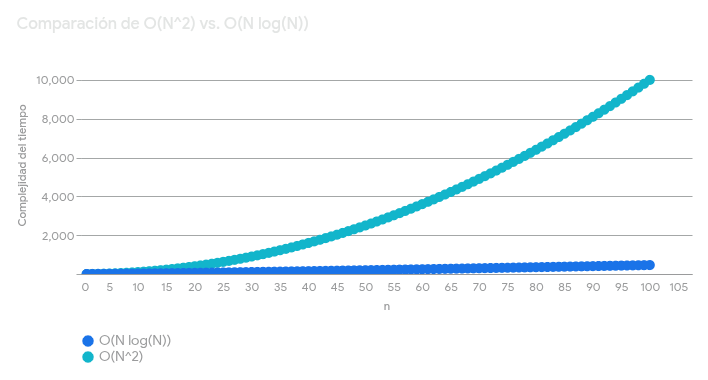
\includegraphics[width=9cm,clip,trim=30 0 0 50]{Figures/ON2_vs_ON_logN.png}
    
    \end{itemize}
\end{frame}


\begin{frame}
  \frametitle{Cómputo eficiente de la respuesta del sistema FIR}  
  \begin{itemize}
    \item Respuesta de un sistema FIR: podemos usar el producto de DFTs.
    \begin{itemize}
      \item Suponemos $x[n]$ de longitud L y $h[n]$ de longitud M.
      \item Con $L$ o $M$ elevadas, el cálculo debe ser eficiente (FFT).    
    \end{itemize}


    \item Si $L>>M$ se puede simplificar el calculo.
    \begin{itemize}
      \item Se divide $x[n]$ en subsecuencias de $L_D+M-1$ valores, $L_D>>M$.
      \item Método 1: solapamiento y almacenamiento.
      \item Método 2: solapamiento y suma.
    \end{itemize}
  \end{itemize}
  
\end{frame}
  
  
\begin{frame}
  \frametitle{Representación de la DFT}
  
  \footnotesize
  \begin{itemize}  
    \item DFT: \color{blue}{\texttt{X=fft(x)}}\color{black}, IDFT: \color{blue}{\texttt{x=ifft(X)}}
    \begin{itemize}
      \footnotesize
      \item \color{blue}{\textrm{x}} \color{black} es un vector con \color{blue}{\textrm{N=length(x)}} \color{black} elementos,
      \item \color{blue}{\textrm{X}} \color{black} es su DFT con \color{blue}{\texttt{N}} \color{black}  elementos.
      \item Para obtener más muestras de la DFT, rellenamos \color{blue}{\texttt{x}} \color{black}con ceros.
      \item Representamos el modulo y el argumento por separado.
      \item Para representarlo frente a $\Omega$ discreta:
      \begin{itemize}
        \item \color{blue}{\texttt{w=2*pi*[0:N-1]/N}};\color{black} (rad/muestra) 
        \item \color{blue}{\texttt{f=[0:N-1]/N}};\color{black}  (1/muestra)
        \item \color{blue}{\texttt{f=2*[0:N-1]/N}};\color{black} (frec. normalizada) 
      \end{itemize}
      \item Para representarlo frente a $\omega$ continua:
      \begin{itemize}
        \item \color{blue}{\texttt{w=2*pi*[0:N-1]/N/Ts}};\color{black}(rad/s) 
        \item \color{blue}{\texttt{f=[0:N-1]/N/Ts}};\color{black} (Hz)
      \end{itemize}
    \end{itemize}    
  \end{itemize}
\end{frame}

 
\section{Conclusiones}
\begin{frame}{Conclusiones}
\frametitle{Resumen}
  \begin{itemize}
    \item \alert{FFT - Diezmado temporal en base 2:}
    \begin{itemize}
      \item Divide sucesivamente en subsecuencias pares e impares.
      \item La operación mariposa combina los resultados de las subsecuencias.
      \[\color{blue}
      X[k] = 
      \begin{cases}
        X[k]=F[k] + W_N^k G[k]~\text{para}~k=\{0,...,N/2-1\}\\
        X[k]=F[k] - W_N^{k} G[k]~\text{para}~k=\{N/2,...,N-1\}
      \end{cases}
      \]
      \item Reduce la complejidad de \(O(N^2)\) a \(O(N \log_2 N)\).
    \end{itemize}
    \item \alert{Representación:}
    \begin{itemize}
      \item Frente a $\Omega$ discreta:
      \begin{itemize}
        \item \color{blue}{\texttt{w=2*pi*[0:N-1]/N}};\color{black} (rad/muestra) 
        \item \color{blue}{\texttt{f=[0:N-1]/N}};\color{black}  (1/muestra)
        \item \color{blue}{\texttt{f=2*[0:N-1]/N}};\color{black} (frec. normalizada) 
      \end{itemize}
      \item Frente a $\omega$ continua:
      \begin{itemize}
        \item \color{blue}{\texttt{w=2*pi*[0:N-1]/N/Ts}};\color{black}(rad/s) 
        \item \color{blue}{\texttt{f=[0:N-1]/N/Ts}};\color{black} (Hz)
      \end{itemize}
  \end{itemize}
    \end{itemize}

\end{frame}


\end{document}